% %\documentclass[handout]{beamer}
% \documentclass[evncountsect]{beamer}
% \usepackage{amsmath,algorithm,algorithmic,graphicx,amsfonts,amsthm,color,pgf,tikz,wrapfig,amsfonts,multicol,wasysym,animate}
% \usepackage[absolute,overlay]{textpos}
% \usetikzlibrary{arrows}
% \beamertemplatenavigationsymbolsempty
% \setbeamercovered{transparent = 0}
% \useoutertheme[subsection=false]{miniframes}
% \bibliographystyle{apalike}
% \setlength{\fboxrule}{1pt}
\documentclass[professionalfont, 12pt, default]{beamer}
% available at https://github.com/matze/mtheme
% should be found in /usr/share/texlive/texmf-dist/tex/latex/beamertheme-metropolis
\beamertemplatenavigationsymbolsempty
\setbeamercovered{transparent = 0}
%\setbeamercovered{dynamic} % slightly displaying not highlight
\useoutertheme[subsection=false]{miniframes}
\usetheme{metropolis}

\usepackage{mathpazo}
\usepackage{longtable}
%\usepackage[fontset=windowsnew,UTF8]{ctex}

%\setbeamertemplate{footline}[page number]

\setbeamercolor{structure}{fg=white!20!gray}
\mathversion{bold}
\usepackage{graphicx}
\usepackage{amsmath, amssymb, cite, url}
\usepackage{etex}

% Comment these out if you don't want a slide with just the
% part/section/subsection/subsubsection title:
% \AtBeginPart{\frame{\partpage}}
% \AtBeginSection{\frame{\sectionpage}}
% \AtBeginSubsection{\frame{\subsectionpage}}
% \AtBeginSubsubsection{\frame{\subsubsectionpage}}
\setlength{\parindent}{0pt}
% \setlength{\parskip}{6pt plus 2pt minus 1pt}
\setlength{\emergencystretch}{3em}  % prevent overfull lines
\setcounter{secnumdepth}{0}

\title{A compendium of RNA-binding motifs for decoding gene regulation}
\author{Ray D., et al. Nature, 2013, vol.~499, pp.~172-177}
\date{\today}

\InputIfFileExists{macro.tex}{}{}
% macro
\def\BeginColumn#1{\begin{columns}\column{#1\textwidth}}
\def\Column#1{\column{#1\textwidth}}
\def\EndColumn{\end{columns}}
\providecommand{\tightlist}{%
    \setlength{\itemsep}{0pt}\setlength{\parskip}{0pt}}

\begin{document}
\frame{\titlepage}

\section{Introduction}\label{introduction}

\begin{frame}{RNA-binding proteins (RBPs)}

\begin{itemize}
\tightlist
\item
  Are proteins binding to double or single stranded RNA in cells.
\item
  Regulate numerous aspect of co- and post-transcriptional gene
  expression

  \begin{itemize}
  \tightlist
  \item
    RNA splicing, capping, polyadenylation, mRNA export, etc.
  \end{itemize}
\end{itemize}

\end{frame}

\begin{frame}{Figure 1}

\begin{figure}
\centering
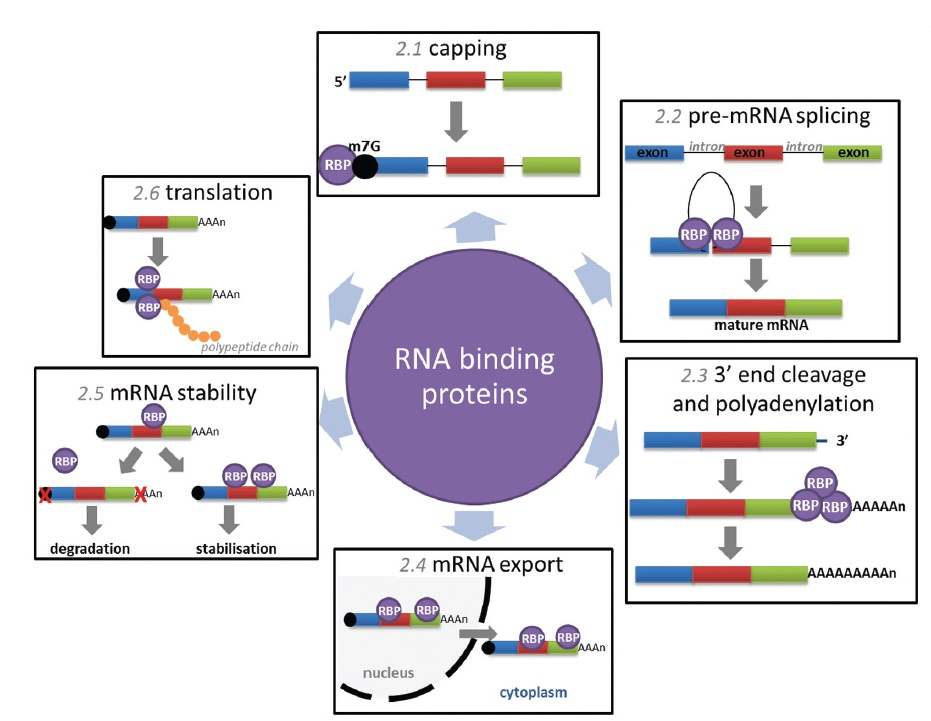
\includegraphics[width=0.80000\textwidth]{img/RBPs1.jpg}
\caption{Sutherland JM., et al. Asian J Androl 2015}
\end{figure}

\end{frame}

\begin{frame}{RNA-binding domains (RBDs)}

\begin{block}{Functions}

\begin{itemize}
\tightlist
\item
  Recognize RNA: bind short, single-stranded RNA sequences, or
  structured RNAs.
\end{itemize}

\end{block}

\begin{block}{Types}

\begin{itemize}
\tightlist
\item
  RNA recognition motif, hnRNP K-homology (KH), zinc finger domains,
  etc.
\end{itemize}

\end{block}

\end{frame}

\begin{frame}{Post-transcriptional regulation}

\begin{itemize}
\tightlist
\item
  Contributes substantially to gene expression across human tissues.
\end{itemize}

However,

\begin{itemize}
\tightlist
\item
  Lack of motifs for the vast majority of RBPs across all branches of
  eukaryotes.

  \begin{itemize}
  \tightlist
  \item
    Due to higher flexibility of the RNA-protein interface for major
    types of BRPs;
  \item
    Example: only 15\% of human RBD-containing proteins have known
    RNA-binding motifs.
  \end{itemize}
\end{itemize}

\textbf{This paper: identifies binding motifs for a broad range of RBPs}

\end{frame}

\section{Methods}\label{methods}

\begin{frame}{\texttt{RNAcompete} experiments}

\begin{itemize}
\tightlist
\item
  An \emph{in vitro} method for the analysis of RNA binding preferences
  of hundreds of RBD-containing RBPs, from diverse eukaryotes.
\item
  Rely on binding reaction between RBD and RNA-binding motifs.

  \begin{itemize}
  \tightlist
  \item
    An RBP is incubated in a complex pool of RNAs by affinity selection.
  \item
    The pool contains \textasciitilde{}240,000 short RNAs, divided into
    two halves for internal cross-validation purpose.
  \end{itemize}
\item
  The associated RNAs are interrogated by microarray and computational
  analyses.
\end{itemize}

\end{frame}

\begin{frame}{Figure 2}

\begin{figure}
\centering
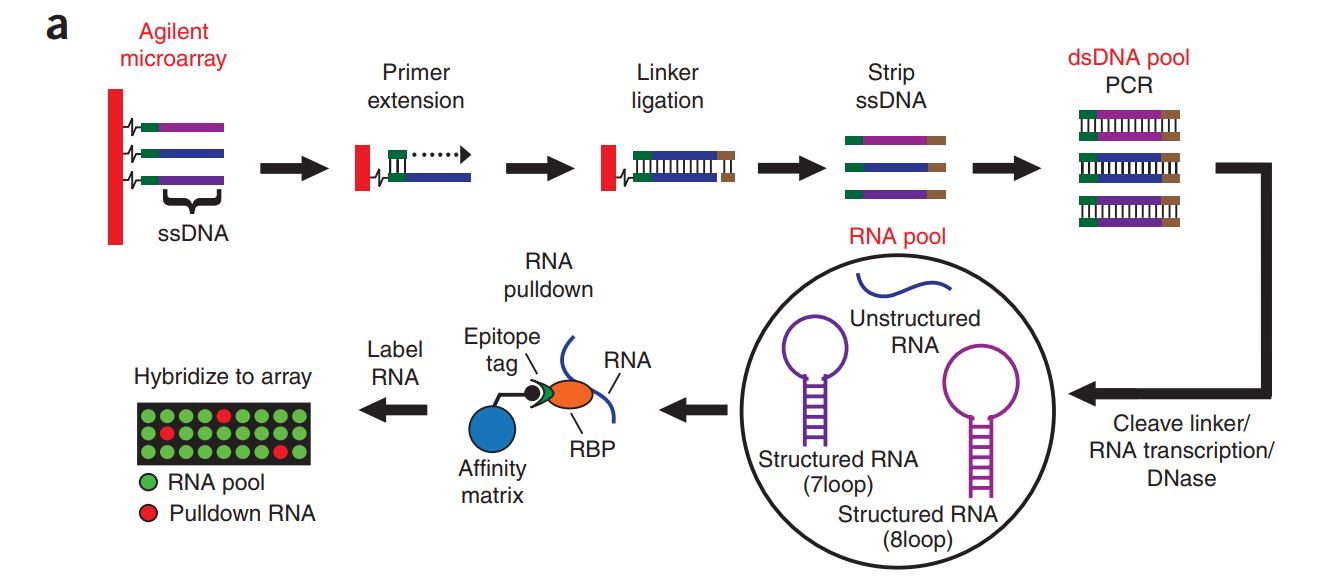
\includegraphics[width=0.80000\textwidth]{img/RNAcompete.png}
\caption{Ray D., et al. Nature 2009, Fig 1}
\end{figure}

\end{frame}

\section{Results}\label{results}

\begin{frame}{Large-scale analysis of RBPs}

Determined sequence preferences for 207 RBPs (from 193 unique
RBP-encoding genes), 85 from human.

\begin{itemize}
\tightlist
\item
  Most RBDs fundamentally recognize and bind ssRNA, requires rarely on
  RNA second structure.

  \begin{itemize}
  \tightlist
  \item
    Fig. 1a: Z score and motifs for ZC3H10 (no previously known motif)
  \end{itemize}
\item
  Highlight specificity and diversity of RBP sequence preferences.

  \begin{itemize}
  \tightlist
  \item
    Fig. 1b: E score (enrichment score, Berger MF, et al., Nature
    Biotech 2006)
  \end{itemize}
\item
  The RNAcompete motif substantially outperforms the literature motif by
  AUROC analysis.

  \begin{itemize}
  \tightlist
  \item
    Fig. 1c: AUROC
  \end{itemize}
\end{itemize}

\end{frame}

\begin{frame}{Figure 3}

\begin{figure}
\centering
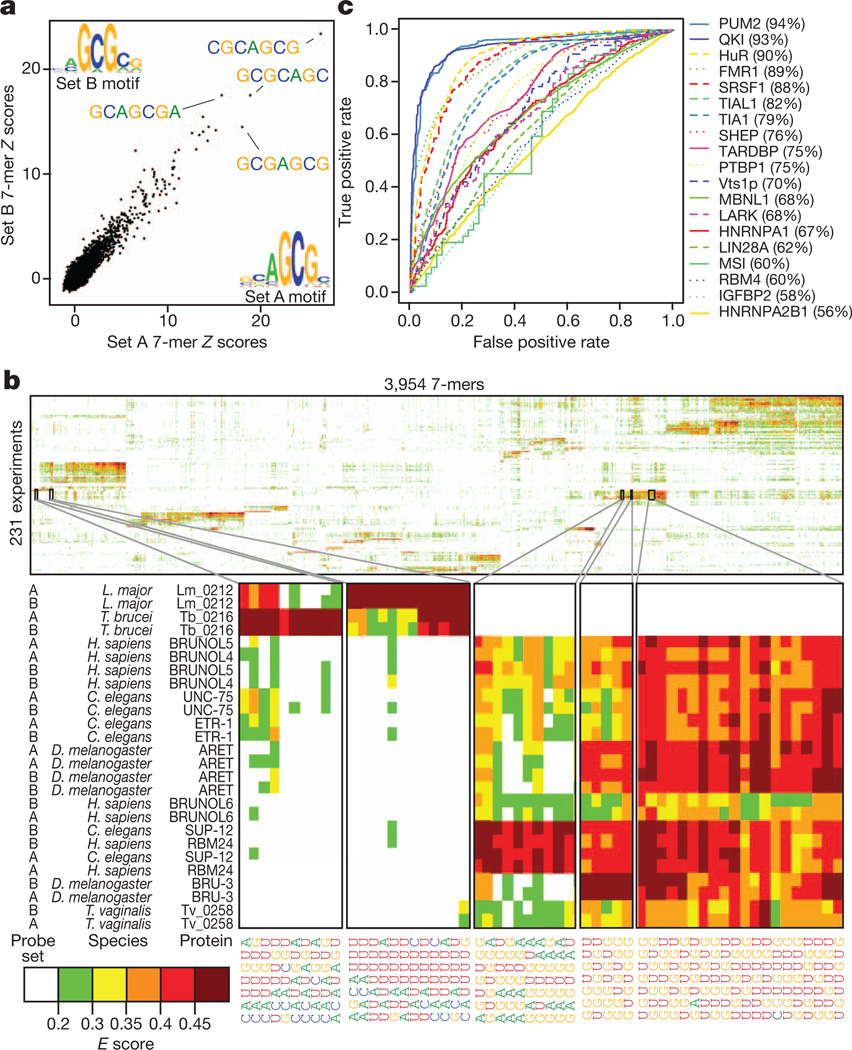
\includegraphics[width=0.60000\textwidth]{img/f1.jpg}
\caption{Ray D., et al. Nature 2013, Fig 1}
\end{figure}

\end{frame}

\begin{frame}{Conservation of ancient motifs}

\begin{itemize}
\tightlist
\item
  Groups of ancient RBP families retain closely related sequence
  preferences.

  \begin{itemize}
  \tightlist
  \item
    A2BP1/RBFOX1, BRUNO/ARET
  \item
    all RBPs in the SUP12--RBM24--RBM38 cluster prefer similar
    (G+U)-rich sequences.
  \end{itemize}
\item
  Subtle differences between more distantly related proteins are found.

  \begin{itemize}
  \tightlist
  \item
    family members from fungi, protists and algae maintained the
    presumed ancestral CAC core-recognition specificity17, but differ in
    their preferenceforflanking nucleotides
  \end{itemize}
\end{itemize}

\end{frame}

\begin{frame}{Figure 4}

\begin{figure}
\centering
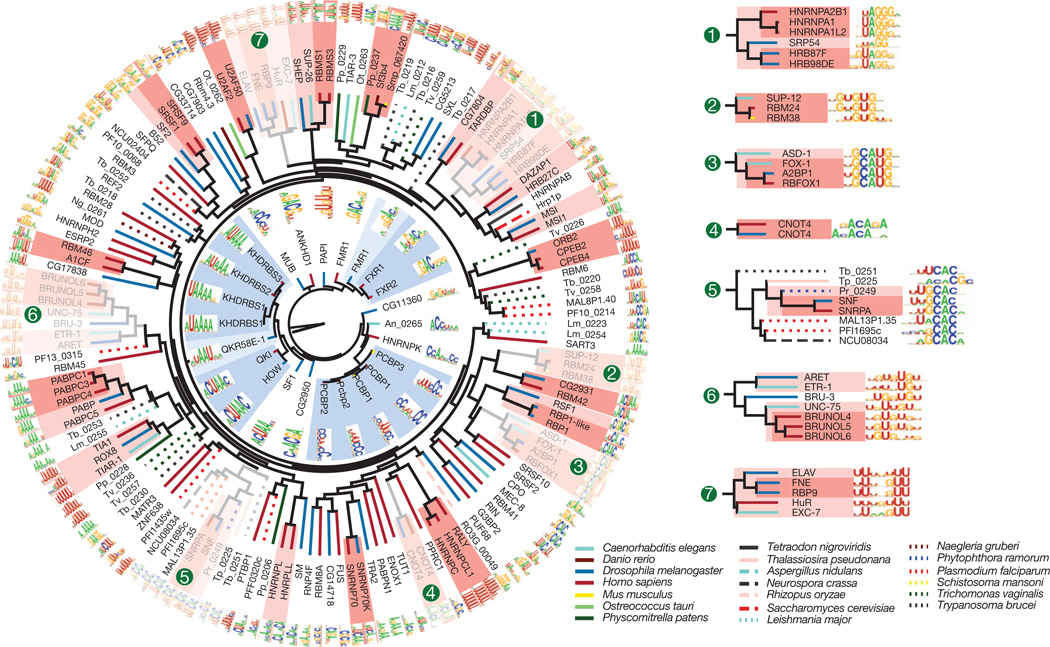
\includegraphics[width=0.90000\textwidth]{img/f2.jpg}
\caption{Ray D., et al. Nature 2013, Fig 2}
\end{figure}

\end{frame}

\begin{frame}{Figure 5}

\begin{itemize}
\tightlist
\item
  Amino acid sequence identity higher than \textasciitilde{}70\% yields
  very similar motifs
\item
  RNAcompete data captured 57\% of all human RBPs contained multiple
  RBDs, assuming 70\% sequence identity
\item
  Validation of motifs predicted for proteins at 61--96\% amino acid
  identity
\end{itemize}

\end{frame}

\begin{frame}{Figure 5}

\begin{figure}
\centering
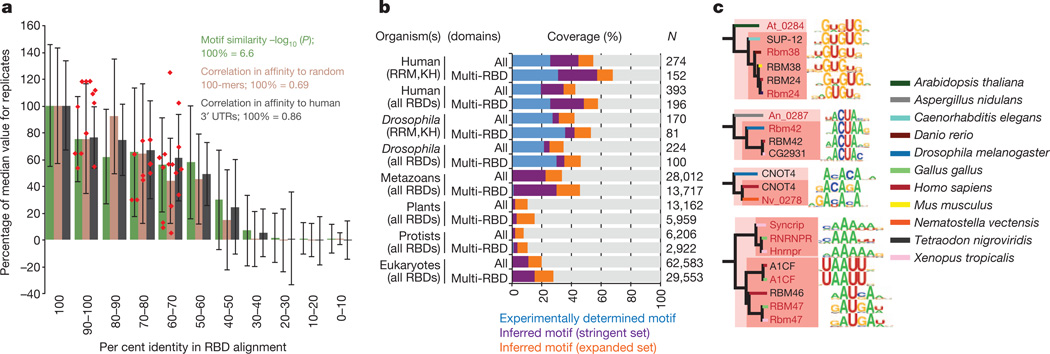
\includegraphics[width=0.90000\textwidth]{img/f3.jpg}
\caption{Ray D., et al. Nature 2013, Fig 3}
\end{figure}

\end{frame}

\begin{frame}{Sequence conservation of motif matches}

\begin{itemize}
\tightlist
\item
  Motifs for most RBP families display significant conservation in one
  or more of the three regions examined.
\end{itemize}

\end{frame}

\begin{frame}{Figure 6}

\begin{figure}
\centering
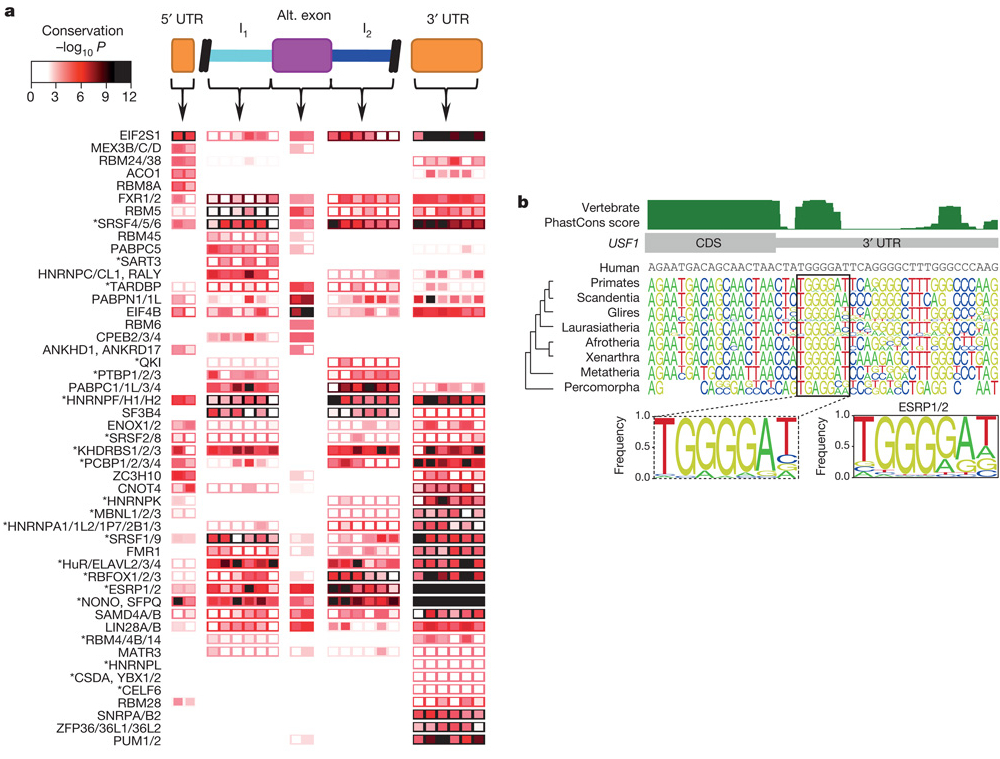
\includegraphics[width=0.70000\textwidth]{img/f4.jpg}
\caption{Ray D., et al. Nature 2013, Fig 4}
\end{figure}

\end{frame}

\begin{frame}{Insights into RBP multi-functionality}

\begin{itemize}
\tightlist
\item
  Role of RBPs in mRNA stability: positive/negative regulator

  \begin{itemize}
  \tightlist
  \item
    For example: RBFOX1 positively regulates mRNA stability/stabilizes
    its predicted mRNA targets
  \end{itemize}
\item
  Reduction of the stability of RBFOX1 targets may affect
  nervous-system-specific processes

  \begin{itemize}
  \tightlist
  \item
    Levels of RBFOX1 in the brains of individuals with autism is
    associated with changes in alternative splicing of exons
  \end{itemize}
\end{itemize}

\end{frame}

\begin{frame}{Figure 7}

\begin{figure}
\centering
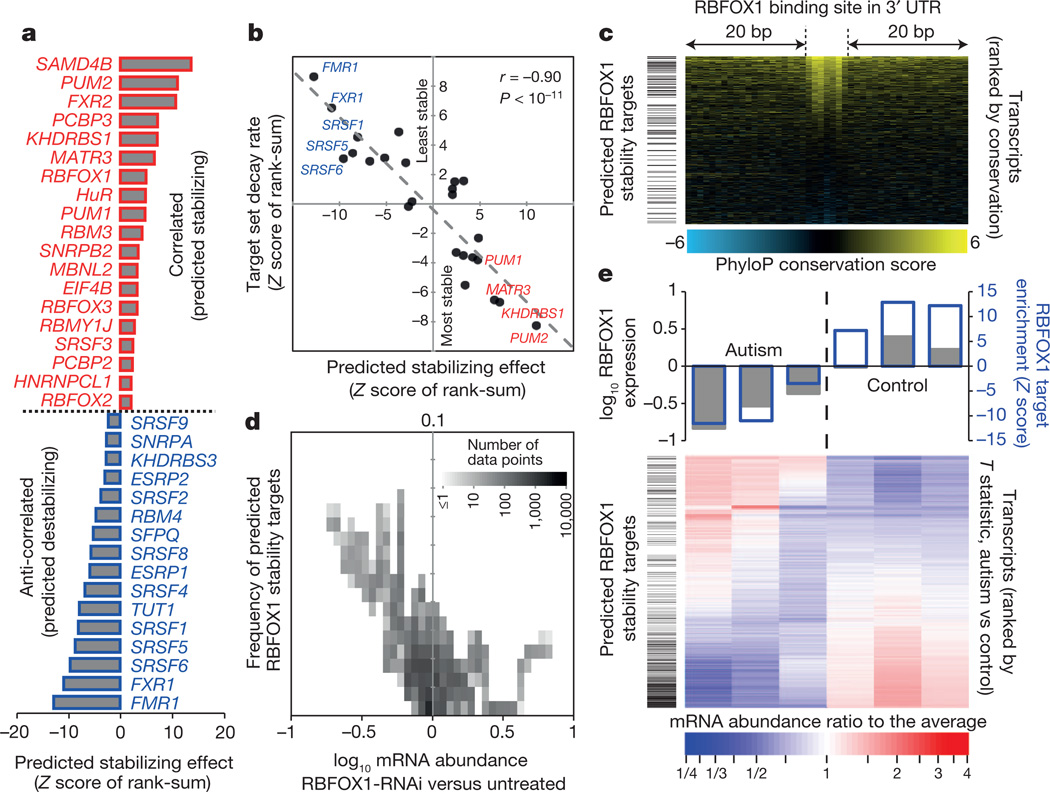
\includegraphics[width=0.70000\textwidth]{img/f5.jpg}
\caption{Ray D., et al. Nature 2013, Fig 5}
\end{figure}

\end{frame}

\section{Discussion}\label{discussion}

\begin{frame}{Significance}

\begin{itemize}
\tightlist
\item
  The resulting motifs represent an unprecedented resource for the
  analysis of post-transcriptional regulation across eukaryotes;
\item
  provide insight into the function and evolution of both RBPs and their
  binding sites;
\item
  reveal broad linkages among different post-transcriptional regulation
  processes;
\item
  uncover an unexpected role for a splicing factor in the control of
  transcript abundance that is mis-regulated in autism.
\end{itemize}

\end{frame}

\end{document}
